\section{矩}
\label{sec:rvm-moments}

均值是$X$的期望，方差是$(X-\mu)^{2}$的期望。把一次方、二次方换成更高的幂，就得到一族数值特征。奖金表与密度$2x$的均值和方差都已算出，但前者向右拖着一个远处的取值，后者的质量堆在右端，这样的形状差别要靠三次、四次的平均来记录。本节先区分几种矩，再讨论它们何时存在、怎样计算，最后用标准化的三阶和四阶矩描述偏斜与尾部，并说明有限个矩能刻画分布到什么程度。

\subsection{定义}
\label{sec:rvm-moment-definition}

幂次不同，平均对偏差的处理方式也不同。奇数次幂保留偏差的符号，正负偏差会相互抵消；偶数次幂和绝对值的幂不分方向，只记偏差的大小。幂次越高，远处的取值占的权重越大：图~\ref{fig:rvm-power-weights}(a)中$\lvert x\rvert^{p}$在$\lvert x\rvert<1$时随$p$增大而变小，在$\lvert x\rvert>1$时随$p$增大而迅速变大。

\begin{definition}[矩]
\label{def:rvm-moments}
设$k$是正整数，$p>0$是实数。
\begin{enumerate}
 \item 若$\mathbb{E}\lvert X\rvert^{k}<\infty$，称
 \begin{equation}
  m_k=\mathbb{E}[X^{k}]
  \label{eq:rvm-raw-moment}
 \end{equation}
 为$X$的$k$阶\term{原点矩}（raw moment）。
 \item 若$\mathbb{E}\lvert X\rvert^{k}<\infty$，记$\mu=\mathbb{E}[X]$，称
 \begin{equation}
  c_k=\mathbb{E}\bigl[(X-\mu)^{k}\bigr]
  \label{eq:rvm-central-moment}
 \end{equation}
 为$X$的$k$阶\term{中心矩}（central moment）。
 \item 称
 \begin{equation}
  \mathbb{E}\lvert X\rvert^{p}\in[0,+\infty]
  \label{eq:rvm-absolute-moment}
 \end{equation}
 为$X$的$p$阶\term{绝对矩}（absolute moment）；$\mathbb{E}\lvert X-\mu\rvert^{p}$称为$p$阶绝对中心矩。
\end{enumerate}
这些量统称为\term{矩}（moment）。
\end{definition}

在这套记号下，均值是$m_1$，方差是$c_2$，并且$c_1=0$。三类矩的存在条件不同。绝对矩是非负变量的期望，总有意义，只是可能为$+\infty$；阶数$p$可以是任意正实数，例如$\mathbb{E}\lvert X\rvert^{1/2}$。原点矩和中心矩是有符号变量的期望，要求相应的绝对矩有限，阶数取正整数，使$x^{k}$对负数也有定义。中心矩还需要先有均值；下一小节将说明，$\mathbb{E}\lvert X\rvert^{k}<\infty$（$k\geq1$）已经保证了均值有限，也保证了$(X-\mu)^{k}$可积。

\begin{BookInlineFigure}
 \centering
 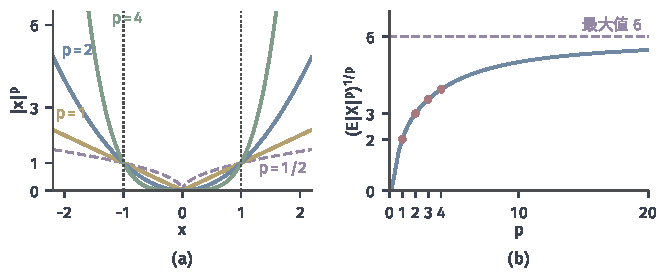
\includegraphics[width=112mm]{figures/07-probability/01-elementary-probability/matplotlib/rvm-power-weights/figure.pdf}
 \caption{幂次与权重。(a)$\lvert x\rvert^{p}$在$p=\tfrac12,1,2,4$时的图像：$\lvert x\rvert<1$时幂次越高权重越小，$\lvert x\rvert>1$时越大，所有曲线在$\lvert x\rvert=1$处（点线）相交。(b)奖金表的$(\mathbb{E}\lvert X\rvert^{p})^{1/p}$随$p$单调增加（蓝），红点是$p=1,2,3,4$时的值$2,3,3.56,3.95$，$p\to\infty$时趋于最大取值$6$（紫色虚线）。}
 \label{fig:rvm-power-weights}
\end{BookInlineFigure}

\paragraph{贯穿例子的矩}
奖金表只取有限个值，各阶矩都存在。由函数期望公式，
\[
 \begin{gathered}
 m_1=2,\qquad m_2=9,\\
 m_3=27\cdot\tfrac13+216\cdot\tfrac16=45,\qquad m_4=81\cdot\tfrac13+1296\cdot\tfrac16=243 .
 \end{gathered}
\]
它的中心矩可以直接从偏差$-2,1,4$计算，例如
\[
 c_3=(-2)^{3}\cdot\tfrac12+1^{3}\cdot\tfrac13+4^{3}\cdot\tfrac16=-4+\tfrac13+\tfrac{32}{3}=7 .
\]
原点矩全为正，因为奖金非负；三阶中心矩为正，是因为偏差$4$的立方$64$远大于偏差$-2$的立方的绝对值$8$，即使后者的概率是前者的三倍。

\subsection{存在性}
\label{sec:rvm-moment-existence}

方差的定义要求$\mathbb{E}[X^{2}]<\infty$，并说明了这一条件蕴含均值有限。同样的道理对一般的阶都成立：高阶矩有限，低阶矩必然有限。

\begin{theorem}[矩的单调存在性]
\label{thm:rvm-moment-monotone}
设$0<p<q$。若$\mathbb{E}\lvert X\rvert^{q}<\infty$，则
\begin{equation}
 \mathbb{E}\lvert X\rvert^{p}\leq1+\mathbb{E}\lvert X\rvert^{q}<\infty .
 \label{eq:rvm-moment-monotone}
\end{equation}
\end{theorem}

\begin{proof}
对每个实数$x$有$\lvert x\rvert^{p}\leq1+\lvert x\rvert^{q}$：若$\lvert x\rvert\leq1$，则$\lvert x\rvert^{p}\leq1$；若$\lvert x\rvert>1$，则$\lvert x\rvert^{p}<\lvert x\rvert^{q}$。把$x$换成$X$并取期望，由保序性即得。
\end{proof}

证明把数轴分成两部分处理。在$\lvert x\rvert\leq1$的近处，所有幂都不超过$1$，总质量又是$1$，所以近处的贡献总是有限的；矩是否存在完全取决于远处，而在远处高次幂压过低次幂。于是$\mathbb{E}\lvert X\rvert^{k}<\infty$蕴含$\mathbb{E}\lvert X\rvert<\infty$，均值存在；再由不等式
\[
 \lvert x-\mu\rvert^{k}\leq2^{k-1}\bigl(\lvert x\rvert^{k}+\lvert\mu\rvert^{k}\bigr),
\]
$(X-\mu)^{k}$也可积，中心矩$c_k$有定义。最后这个不等式来自$t\mapsto t^{k}$在$[0,\infty)$上的凸性。对$a,b\geq0$，凸性给出
\[
 \Bigl(\frac{a+b}{2}\Bigr)^{k}\leq\frac{a^{k}+b^{k}}{2},
\]
再取$a=\lvert x\rvert$，$b=\lvert\mu\rvert$，并利用$\lvert x-\mu\rvert\leq a+b$，两边乘$2^{k}$即得。

\paragraph{定量的比较}
式~\eqref{eq:rvm-moment-monotone}只说明存在，常数$1$也比较粗糙。用Jensen不等式可以得到一个精确的比较：把各阶绝对矩开相应次方，化成同一单位后，它们随阶数单调增加。

\begin{theorem}[Lyapunov不等式]
\label{thm:rvm-lyapunov}
设$0<p<q$且$\mathbb{E}\lvert X\rvert^{q}<\infty$。则
\begin{equation}
 \bigl(\mathbb{E}\lvert X\rvert^{p}\bigr)^{1/p}\leq\bigl(\mathbb{E}\lvert X\rvert^{q}\bigr)^{1/q} .
 \label{eq:rvm-lyapunov}
\end{equation}
\end{theorem}

\begin{proof}
令$r=q/p>1$，$Y=\lvert X\rvert^{p}$。由定理~\ref{thm:rvm-moment-monotone}，$Y$可积，而$\lvert Y\rvert^{r}=\lvert X\rvert^{q}$也可积。函数$f(t)=\lvert t\rvert^{r}$在整个$\mathbb{R}$上是凸函数，由Jensen不等式，
\[
 \bigl(\mathbb{E}[Y]\bigr)^{r}\leq\mathbb{E}\bigl[Y^{r}\bigr],
\]
其中$\mathbb{E}[Y]=\mathbb{E}\lvert X\rvert^{p}$，$\mathbb{E}[Y^{r}]=\mathbb{E}\lvert X\rvert^{q}$。两边开$q$次方，左边成为$(\mathbb{E}\lvert X\rvert^{p})^{1/p}$，即得式~\eqref{eq:rvm-lyapunov}。
\end{proof}

式~\eqref{eq:rvm-lyapunov}称为\term{Lyapunov不等式}（Lyapunov's inequality）。对奖金表，
\[
 \begin{gathered}
 \mathbb{E}\lvert X\rvert=2,\qquad (\mathbb{E}X^{2})^{1/2}=3,\\
 (\mathbb{E}X^{3})^{1/3}=45^{1/3}\approx3.56,\qquad (\mathbb{E}X^{4})^{1/4}=243^{1/4}\approx3.95 .
 \end{gathered}
\]
图~\ref{fig:rvm-power-weights}(b)画出了整条曲线。阶数越高，平均越看重大的取值，最终趋于最大取值$6$：这是因为只保留取值$6$那一项、或把每个取值都放大到$6$，得到
\[
 \tfrac16\cdot6^{p}\leq\mathbb{E}\lvert X\rvert^{p}\leq6^{p},
\]
开$p$次方后左边是$6\cdot6^{-1/p}$，它在$p\to\infty$时趋于$6$。

\paragraph{反方向不成立}
低阶矩有限不能推出高阶矩有限。考虑一族尾部按幂律衰减的密度
\[
 f_X(x)=\alpha x^{-\alpha-1},\qquad x\geq1,
\]
其中$\alpha>0$。它的总质量是$\bigl[-x^{-\alpha}\bigr]_1^{\infty}=1$。对$p>0$，
\[
 \mathbb{E}[X^{p}]=\int_1^{\infty}\alpha x^{p-\alpha-1}\,\mathrm{d}x
 =\begin{cases}\dfrac{\alpha}{\alpha-p}, & p<\alpha,\\ +\infty, & p\geq\alpha .\end{cases}
\]
被积函数是$x$的$p-\alpha-1$次幂，它在无穷远处可积当且仅当指数小于$-1$，即$p<\alpha$。

取$\alpha=3$，均值是$\tfrac32$，$\mathbb{E}[X^{2}]=3$，方差是$3-\tfrac94=\tfrac34$，但三阶矩是$+\infty$。图~\ref{fig:rvm-moment-existence}画出了截断到$[1,M]$的矩：$p=1,2$时分别趋于$\tfrac32$与$3$，$p=3$时等于$3\ln M$，无界增长。取$\alpha=\tfrac32$，均值是$3$而方差无穷；取$\alpha=1$，连均值都是$+\infty$。参数$\alpha$恰好是使矩存在的阶数的上界，它刻画了尾部的厚薄。

\begin{BookInlineFigure}
 \centering
 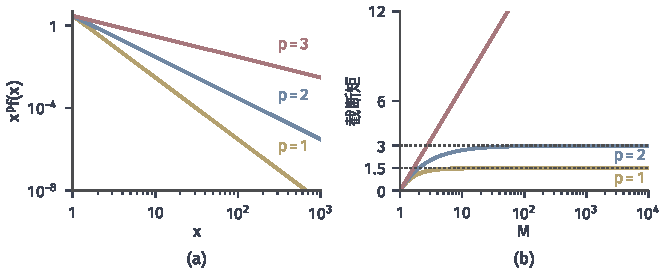
\includegraphics[width=112mm]{figures/07-probability/01-elementary-probability/matplotlib/rvm-moment-existence/figure.pdf}
 \caption{密度$f(x)=3x^{-4}$（$x\geq1$）的矩。(a)双对数坐标下的被积函数$x^{p}f(x)=3x^{p-4}$是直线，斜率为$p-4$；$p=3$时斜率为$-1$，衰减不足以使积分有限。(b)截断矩$\int_1^{M}x^{p}f(x)\,\mathrm{d}x$：$p=1$（黄）与$p=2$（蓝）分别趋于$1.5$与$3$（点线），$p=3$（红）按$3\ln M$增长。}
 \label{fig:rvm-moment-existence}
\end{BookInlineFigure}

离散的例子也一样。第~\ref{sec:rvm-expectation-definition}小节的$p_X(k)=1/[k(k+1)]$满足$k^{p}p_X(k)\leq k^{p-2}$，所以$p<1$时$\mathbb{E}[X^{p}]$有限，而均值是$+\infty$。下表把这些要求的强弱排在一起，每一行的条件蕴含它上面各行的条件。

\begin{BookInlineTable}
 \centering
 \caption{有限矩的要求，以$f(x)=\alpha x^{-\alpha-1}$（$x\geq1$）为例。}
 \label{tab:rvm-moment-requirements}
 \begin{tabular}{lll}
  \toprule
  要求 & 条件 & 使之成立的$\alpha$\\
  \midrule
  均值有限 & $\mathbb{E}\lvert X\rvert<\infty$ & $\alpha>1$\\
  方差有限 & $\mathbb{E}[X^{2}]<\infty$ & $\alpha>2$\\
  偏度有定义 & $\mathbb{E}\lvert X\rvert^{3}<\infty$ & $\alpha>3$\\
  峰度有定义 & $\mathbb{E}[X^{4}]<\infty$ & $\alpha>4$\\
  \bottomrule
 \end{tabular}
\end{BookInlineTable}

\subsection{计算}
\label{sec:rvm-moment-computation}

计算矩就是对幂函数使用函数期望公式，再逐项检查可积性。对密度$2x$，
\[
 m_k=\int_0^1x^{k}\cdot2x\,\mathrm{d}x=\frac{2}{k+2},
\]
于是$m_1=\tfrac23$，$m_2=\tfrac12$，$m_3=\tfrac25$，$m_4=\tfrac13$。直接计算中心矩要展开$(x-\tfrac23)^{k}$再积分，比较繁琐。更好的办法是先算原点矩，再用二项式展开换算。

\begin{theorem}[原点矩与中心矩的换算]
\label{thm:rvm-moment-conversion}
设$k$是正整数，$\mathbb{E}\lvert X\rvert^{k}<\infty$，$\mu=m_1$，并约定$m_0=c_0=1$。则
\begin{align}
 c_k&=\sum_{j=0}^{k}\binom{k}{j}m_j\,(-\mu)^{k-j},
 \label{eq:rvm-central-from-raw}\\
 m_k&=\sum_{j=0}^{k}\binom{k}{j}c_j\,\mu^{k-j}.
 \label{eq:rvm-raw-from-central}
\end{align}
\end{theorem}

\begin{proof}
由定理~\ref{thm:rvm-moment-monotone}，$j\leq k$时$\mathbb{E}\lvert X\rvert^{j}<\infty$，各$m_j$都是有限数。对$(X-\mu)^{k}$用二项式定理，
\[
 (X-\mu)^{k}=\sum_{j=0}^{k}\binom{k}{j}X^{j}(-\mu)^{k-j},
\]
右边是有限个可积变量的线性组合，由线性性逐项取期望得式~\eqref{eq:rvm-central-from-raw}。把$X$写成$(X-\mu)+\mu$再展开，同样得到式~\eqref{eq:rvm-raw-from-central}。
\end{proof}

$k=2$时式~\eqref{eq:rvm-central-from-raw}就是方差展开式$c_2=m_2-\mu^{2}$。$k=3,4$时，代入$m_1=\mu$并合并同类项，得到
\[
 c_3=m_3-3\mu m_2+2\mu^{3},\qquad c_4=m_4-4\mu m_3+6\mu^{2}m_2-3\mu^{4} .
\]

用这两个式子重算奖金表，$\mu=2$。三阶中心矩是
\[
 c_3=45-3\cdot2\cdot9+2\cdot8=7,
\]
与按偏差计算的结果一致。四阶中心矩是
\[
 c_4=243-4\cdot2\cdot45+6\cdot4\cdot9-3\cdot16=243-360+216-48=51 .
\]
对密度$2x$，$\mu=\tfrac23$，代入$m_2=\tfrac12$，$m_3=\tfrac25$，$m_4=\tfrac13$，通分到分母$135$，得到
\[
 c_3=\tfrac25-1+\tfrac{16}{27}=-\tfrac{1}{135},\qquad
 c_4=\tfrac13-\tfrac{16}{15}+\tfrac{4}{3}-\tfrac{16}{27}=\tfrac{1}{135} .
\]
这里$c_4$的四项依次是$m_4$、$4\mu m_3=\tfrac{16}{15}$、$6\mu^{2}m_2=\tfrac43$与$3\mu^{4}=\tfrac{16}{27}$。

\paragraph{平移与缩放}
设$Y=aX+b$。偏差$Y-\mathbb{E}[Y]=a(X-\mu)$与$b$无关，所以中心矩只按缩放变化：
\begin{equation}
 c_k(aX+b)=a^{k}c_k(X),\qquad \mathbb{E}\bigl\lvert Y-\mathbb{E}[Y]\bigr\rvert^{p}=\lvert a\rvert^{p}\,\mathbb{E}\lvert X-\mu\rvert^{p} .
 \label{eq:rvm-central-affine}
\end{equation}
奇数阶中心矩在$a<0$时变号，反映了反射把右侧的偏斜变到左侧。原点矩则随平移改变，$\mathbb{E}[(X+b)^{k}]$按二项式展开是$b$的$k$次多项式。

图~\ref{fig:rvm-raw-central}对奖金表画出了这两种行为。由二项式展开，
\[
 \mathbb{E}[(X+b)^{2}]=9+4b+b^{2},\qquad \mathbb{E}[(X+b)^{3}]=45+27b+6b^{2}+b^{3}
\]
都随$b$变化，而二阶、三阶中心矩始终是$5$与$7$。$b=-\mu=-2$时原点矩与中心矩重合，因为这时$X+b$的均值恰为零。中心矩描述的是质量绕重心的分布，与重心放在数轴何处无关。

\begin{BookInlineFigure}
 \centering
 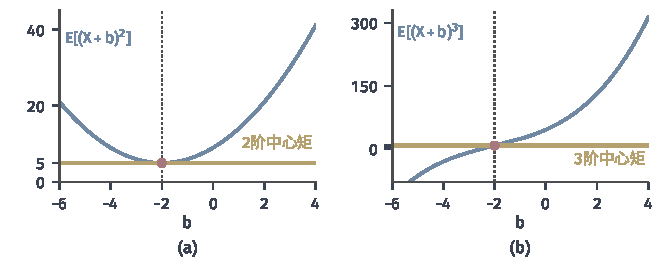
\includegraphics[width=112mm]{figures/07-probability/01-elementary-probability/matplotlib/rvm-raw-central/figure.pdf}
 \caption{平移对原点矩与中心矩的不同影响。对奖金表$X$和平移量$b$：(a)$\mathbb{E}[(X+b)^{2}]$（蓝）是$b$的二次函数，二阶中心矩（黄）恒为$5$；(b)$\mathbb{E}[(X+b)^{3}]$（蓝）是$b$的三次函数，三阶中心矩（黄）恒为$7$。两者在$b=-2$（红点）相交。}
 \label{fig:rvm-raw-central}
\end{BookInlineFigure}

\paragraph{形式展开的陷阱}
换算公式的前提是$\mathbb{E}\lvert X\rvert^{k}<\infty$。缺少这一条时，按形式展开或凭对称性写出的数可能毫无意义。考虑对称的密度
\[
 f_X(x)=\frac{3}{2x^{4}},\qquad \lvert x\rvert\geq1 .
\]
它两侧各有质量$\tfrac12$，均值为$0$，方差是
\[
 \mathbb{E}[X^{2}]=2\int_1^{\infty}x^{2}\cdot\frac{3}{2x^{4}}\,\mathrm{d}x=3\int_1^{\infty}x^{-2}\,\mathrm{d}x=3 .
\]

三阶矩却没有定义：$X^{3}$的正部期望是
\[
 \int_1^{\infty}x^{3}\cdot\frac{3}{2x^{4}}\,\mathrm{d}x=\frac32\int_1^{\infty}\frac{\mathrm{d}x}{x}=+\infty,
\]
负部也是$+\infty$。密度对称会诱使人写下“奇数阶矩为零”，但这只在相应的绝对矩有限时成立，此时被积函数是可积的奇函数。这里$\mathbb{E}\lvert X\rvert^{3}=+\infty$，三阶中心矩和下一小节的偏度都不存在。凡是使用矩的公式，都要先确认它所涉及的最高阶绝对矩有限。

\subsection{偏度与峰度}
\label{sec:rvm-skewness-kurtosis}

三阶中心矩的正负反映偏斜方向，但它的数值带着单位：奖金以元计时$c_3=7$，改用角计时变成$7000$。式~\eqref{eq:rvm-central-affine}说明$c_k$按$a^{k}$缩放，除以$\sigma^{k}$就消去了尺度。等价地，先标准化再求矩。

\begin{definition}[偏度与峰度]
\label{def:rvm-skewness-kurtosis}
设$0<\operatorname{Var}(X)=\sigma^{2}<\infty$，$\mu=\mathbb{E}[X]$，$Z=(X-\mu)/\sigma$。若$\mathbb{E}\lvert X\rvert^{3}<\infty$，称
\begin{equation}
 \gamma_1=\frac{c_3}{\sigma^{3}}=\mathbb{E}[Z^{3}]
 \label{eq:rvm-skewness}
\end{equation}
为$X$的\term{偏度}（skewness）。若$\mathbb{E}[X^{4}]<\infty$，称
\begin{equation}
 \kappa=\frac{c_4}{\sigma^{4}}=\mathbb{E}[Z^{4}]
 \label{eq:rvm-kurtosis}
\end{equation}
为$X$的\term{峰度}（kurtosis），称$\kappa-3$为\term{超额峰度}（excess kurtosis）。
\end{definition}

由式~\eqref{eq:rvm-central-affine}，对$a>0$，$aX+b$与$X$的偏度和峰度都相同；对$a<0$，偏度变号，峰度不变。超额峰度减去的$3$，是下一章将要介绍的高斯分布的峰度。不同文献对“峰度”一词有时指$\kappa$、有时指$\kappa-3$，读数之前要先确认约定。这里讨论的是给定分布的总体量；由观测数据估计偏度和峰度属于统计推断。

两个贯穿例子的值如下。奖金表的
\[
 \gamma_1=\frac{7}{5^{3/2}}\approx0.626,\qquad \kappa=\frac{51}{25}=2.04 .
\]
密度$2x$的方差是$\tfrac{1}{18}$，$\sigma^{3}=1/(54\sqrt2)$，$\sigma^{4}=\tfrac{1}{324}$，于是
\[
 \gamma_1=-\frac{54\sqrt2}{135}=-\frac{2\sqrt2}{5}\approx-0.566,\qquad \kappa=\frac{324}{135}=\frac{12}{5} .
\]
奖金表的偏度为正：远处那个$6$元在均值右侧，立方把它的影响放大。密度$2x$的质量堆在右端，左侧有一条渐渐变薄的长边，偏度为负。

\paragraph{零偏度不保证对称}
若$X$关于$\mu$对称且$\mathbb{E}\lvert X\rvert^{3}<\infty$，则$(X-\mu)^{3}$与$-(X-\mu)^{3}$同分布，$c_3=-c_3$，偏度为零。反过来不成立。设$Y$以概率$\tfrac16,\tfrac12,\tfrac13$取$-5,-1,4$。它的均值和三阶矩分别是
\[
 \mathbb{E}[Y]=-\tfrac56-\tfrac12+\tfrac43=0,\qquad
 \mathbb{E}[Y^{3}]=-\tfrac{125}{6}-\tfrac12+\tfrac{64}{3}=0 .
\]
所以$c_3=0$，偏度为零。但$Y$不对称：取负值的概率是$\tfrac23$，中位数是$-1$而不是均值$0$。图~\ref{fig:rvm-zero-skew}显示，零偏度只是左侧一个远偏差的立方与右侧一个中等偏差的立方恰好抵消。

\begin{BookInlineFigure}
 \centering
 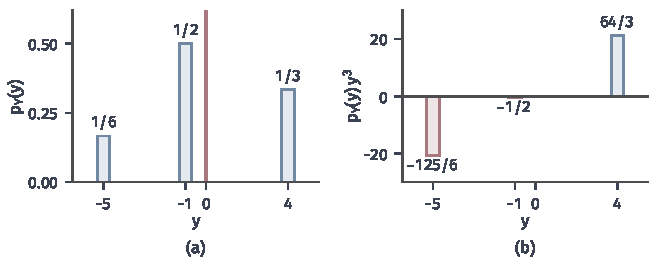
\includegraphics[width=112mm]{figures/07-probability/01-elementary-probability/matplotlib/rvm-zero-skew/figure.pdf}
 \caption{偏度为零的不对称分布。(a)$Y$以概率$\tfrac16,\tfrac12,\tfrac13$取$-5,-1,4$，均值为$0$（红线），方差为$10$。(b)三阶矩的各项贡献$p_Y(y)\,y^{3}$：左侧两项（红）之和$-\tfrac{64}{3}$与右侧一项（蓝）$\tfrac{64}{3}$相互抵消。}
 \label{fig:rvm-zero-skew}
\end{BookInlineFigure}

\paragraph{峰度衡量什么}
由标准化变量$Z$的$\mathbb{E}[Z^{2}]=1$，可以把峰度改写成
\[
 \kappa-1=\mathbb{E}[Z^{4}]-\bigl(\mathbb{E}[Z^{2}]\bigr)^{2}=\operatorname{Var}(Z^{2}) .
\]
这给出了峰度的一个准确读法：它衡量$Z^{2}$在其均值$1$周围的波动。若质量都集中在$\lvert Z\rvert=1$附近，$Z^{2}$几乎不变，峰度接近$1$；若一部分质量在中心附近、另一部分在很远处，$Z^{2}$变化剧烈，峰度就大。所以峰度同时受中心附近和远处的影响，不能只理解为峰的尖锐程度。由这个读法还可以得到峰度与偏度之间的约束。

\begin{theorem}[偏度与峰度的约束]
\label{thm:rvm-pearson}
设$\mathbb{E}[X^{4}]<\infty$且$\operatorname{Var}(X)>0$。则
\begin{equation}
 \kappa\geq1+\gamma_1^{2} .
 \label{eq:rvm-pearson}
\end{equation}
对离散的$X$，等号成立当且仅当$X$以概率一只取两个值。
\end{theorem}

\begin{proof}
记$Z$为标准化变量，考虑非负变量$W=(Z^{2}-\gamma_1Z-1)^{2}$。展开后各项都是$Z$的不超过四次的幂，都可积：
\[
 W=Z^{4}-2\gamma_1Z^{3}+(\gamma_1^{2}-2)Z^{2}+2\gamma_1Z+1 .
\]
代入$\mathbb{E}[Z]=0$，$\mathbb{E}[Z^{2}]=1$，$\mathbb{E}[Z^{3}]=\gamma_1$，$\mathbb{E}[Z^{4}]=\kappa$，由线性性得
\[
 0\leq\mathbb{E}[W]=\kappa-2\gamma_1^{2}+\gamma_1^{2}-2+1=\kappa-\gamma_1^{2}-1 .
\]

等号成立当且仅当$\mathbb{E}[W]=0$。对离散的$X$，这等价于$Z$的每个正概率取值都是二次方程$z^{2}-\gamma_1z-1=0$的根。这个方程的判别式$\gamma_1^{2}+4>0$，恰有两个实根，所以$Z$至多取两个值；它的方差为一，不是常数，因此恰好取两个值。反过来，设$Z$只取两个值$z_1<z_2$，概率分别为$1-r$与$r$。由$\mathbb{E}[Z]=0$得$(1-r)z_1=-rz_2$，代入$\mathbb{E}[Z^{2}]=1$，
\[
 1=(1-r)z_1\cdot z_1+rz_2\cdot z_2=-rz_2z_1-(1-r)z_1z_2=-z_1z_2 .
\]
所以$z_1,z_2$是二次方程$z^{2}-(z_1+z_2)z-1=0$的两个根，于是
\[
 z_k^{2}=(z_1+z_2)z_k+1,\qquad k=1,2 .
\]两边乘$z_k$后取期望，得到
\[
 \gamma_1=\mathbb{E}[Z^{3}]=(z_1+z_2)\,\mathbb{E}[Z^{2}]+\mathbb{E}[Z]=z_1+z_2 .
\]于是$Z$的两个取值都满足$z^{2}-\gamma_1z-1=0$，$W$恒为零，等号成立。
\end{proof}

图~\ref{fig:rvm-skew-kurt-plane}把本节的例子放到偏度—峰度平面上。抛物线$\kappa=1+\gamma_1^{2}$下方的区域不可能出现；两点分布恰好落在抛物线上，例如以概率$\tfrac56,\tfrac16$取$1,7$的表，偏度$4/\sqrt5\approx1.79$，峰度$4.2$。三点或更多点的分布与有密度的分布都在抛物线上方。

\begin{BookInlineFigure}
 \centering
 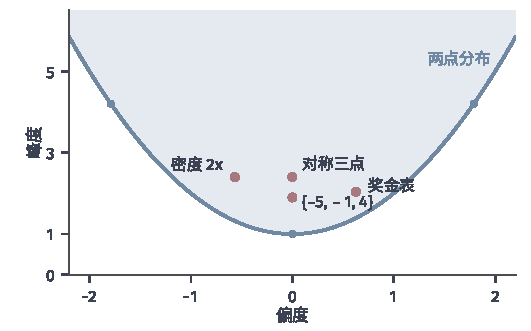
\includegraphics[width=90mm]{figures/07-probability/01-elementary-probability/matplotlib/rvm-skew-kurt-plane/figure.pdf}
 \caption{偏度—峰度平面。可能出现的点位于抛物线$\kappa=1+\gamma_1^{2}$上或其上方（浅蓝区域），两点分布落在抛物线上（蓝点为取值概率$\tfrac16,\tfrac12,\tfrac56$的三例）。红点是本节的例子：奖金表$(0.63,2.04)$，密度$2x$为$(-0.57,2.4)$，$Y$在$\{-5,-1,4\}$上为$(0,1.9)$，对称三点分布为$(0,2.4)$。}
 \label{fig:rvm-skew-kurt-plane}
\end{BookInlineFigure}

\paragraph{峰度不能单独确定形状}
同一个峰度可以对应形状完全不同的分布。设$Z$以概率$q,1-2q,q$取$-a,0,a$。方差为一要求$2qa^{2}=1$，而$\mathbb{E}[Z^{4}]=2qa^{4}=\frac{1}{2q}$。取$q=\tfrac{5}{24}$，峰度是$\tfrac{12}{5}$，与密度$2x$的峰度相同。

图~\ref{fig:rvm-same-kurtosis}把两者并列：一个是向右上升、支撑有界、偏度为负的三角形密度，另一个是对称的三点分布，中间有一个高的质量。两者峰度都是$2.4$，低于$3$。峰度既不能说明峰的尖锐，也不能说明尾部是否有界，它只是$Z^{2}$的波动这一个数。描述尾部的衰减规律要直接看尾概率，第~\ref{chap:tail-probabilities}章会用矩来估计它。

\begin{BookInlineFigure}
 \centering
 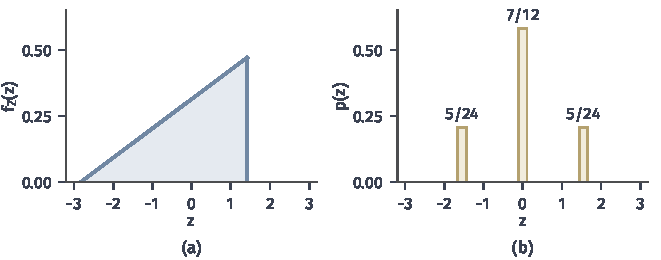
\includegraphics[width=112mm]{figures/07-probability/01-elementary-probability/matplotlib/rvm-same-kurtosis/figure.pdf}
 \caption{峰度相同而形状不同的两个标准化分布。(a)密度$2x$标准化后的三角形密度（蓝），偏度$-0.57$；(b)以概率$\tfrac{5}{24},\tfrac{7}{12},\tfrac{5}{24}$取$-1.55,0,1.55$的对称三点分布（黄），偏度$0$。两者均值为$0$、方差为$1$，峰度都是$12/5$。}
 \label{fig:rvm-same-kurtosis}
\end{BookInlineFigure}

\subsection{矩对分布的刻画}
\label{sec:rvm-moments-characterize}

均值、方差、偏度、峰度一个比一个记录更细的信息。自然要问：知道前几个矩，能否确定分布？如果能，概率表与密度就可以用一串数代替。答案是否定的，而且相差得很远。

\paragraph{均值与方差相同的三张表}
奖金表的均值是$2$，方差是$5$。两点分布的方差有一个简单公式：以概率$1-r$与$r$取$a<b$时，均值$\mu$满足$(1-r)(a-\mu)+r(b-\mu)=0$，方差等于$(b-\mu)(\mu-a)$。要求$\mu=2$、方差为$5$，可取$a=1,b=7$，此时$r=\tfrac16$；也可取$a=-3,b=3$，此时$r=\tfrac56$。

于是三张表以概率$\tfrac12,\tfrac13,\tfrac16$取$0,3,6$，以概率$\tfrac56,\tfrac16$取$1,7$，以概率$\tfrac16,\tfrac56$取$-3,3$，它们的均值都是$2$、方差都是$5$。图~\ref{fig:rvm-same-mean-var}显示它们的形状截然不同：第二张右偏，第三张左偏，偏度分别为$\pm4/\sqrt5\approx\pm1.79$，奖金表的偏度是$0.63$。均值和方差只确定了重心与转动惯量，质量怎样具体分配，它们管不到。

\begin{BookInlineFigure}
 \centering
 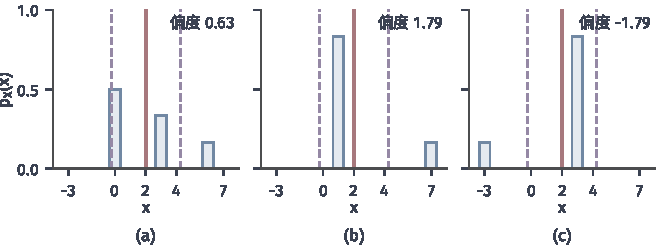
\includegraphics[width=112mm]{figures/07-probability/01-elementary-probability/matplotlib/rvm-same-mean-var/figure.pdf}
 \caption{均值都是$2$（红线）、方差都是$5$的三张概率表，紫色虚线是均值加减标准差$\sqrt5$。(a)奖金表；(b)以概率$\tfrac56,\tfrac16$取$1,7$；(c)以概率$\tfrac16,\tfrac56$取$-3,3$。三者的偏度分别为$0.63$、$1.79$与$-1.79$。}
 \label{fig:rvm-same-mean-var}
\end{BookInlineFigure}

\paragraph{有限个矩不能确定分布}
增加矩的个数也无济于事。只要多给出几个矩，就能用更细的扰动保持它们不变，下面的定理把这一点做成构造。

\begin{theorem}[有限个矩不确定分布]
\label{thm:rvm-finite-moments}
对每个正整数$k$，存在$(0,1)$上的密度$f\neq1$，使以$f$为密度的变量与以常数$1$为密度的变量具有相同的$1,\dots,k$阶矩，而$k+1$阶矩不同。
\end{theorem}

\begin{proof}
寻找次数不超过$k+1$的多项式$q(x)=\sum_{l=0}^{k+1}a_lx^{l}$，使
\begin{equation}
 \int_0^1x^{j}q(x)\,\mathrm{d}x=0,\qquad j=0,1,\dots,k .
 \label{eq:rvm-orthogonal}
\end{equation}
这是关于$k+2$个系数$a_0,\dots,a_{k+1}$的$k+1$个齐次线性方程，未知数多于方程，所以有非零解。非零多项式在$[0,1]$上不恒为零，记$M=\max_{[0,1]}\lvert q\rvert>0$，把$q$换成$q/M$，就可设$\max_{[0,1]}\lvert q\rvert=1$。

令$f=1+q$。它在$(0,1)$上非负，由式~\eqref{eq:rvm-orthogonal}中$j=0$的方程，总积分为一，所以是密度；它不恒等于$1$。对$1\leq j\leq k$，
\[
 \int_0^1x^{j}f(x)\,\mathrm{d}x=\int_0^1x^{j}\,\mathrm{d}x+\int_0^1x^{j}q(x)\,\mathrm{d}x=\int_0^1x^{j}\,\mathrm{d}x,
\]
前$k$阶矩相同。若$k+1$阶矩也相同，则$q$与$1,x,\dots,x^{k+1}$的乘积积分都为零，从而与自身的乘积积分$\int_0^1q^{2}\,\mathrm{d}x=0$，这对非零多项式不可能。
\end{proof}

$k=2$时可以取$q(x)=20x^{3}-30x^{2}+12x-1$。逐项积分可以核对式~\eqref{eq:rvm-orthogonal}：
\[
 \begin{aligned}
 \int_0^1q(x)\,\mathrm{d}x&=5-10+6-1=0,\\
 \int_0^1xq(x)\,\mathrm{d}x&=4-\tfrac{15}{2}+4-\tfrac12=0,\\
 \int_0^1x^{2}q(x)\,\mathrm{d}x&=\tfrac{10}{3}-6+3-\tfrac13=0 .
 \end{aligned}
\]
它在$[0,1]$上的最大绝对值是$1$，在两个端点取到。于是$f=1+q$与常数密度有相同的均值$\tfrac12$和方差$\tfrac1{12}$，三阶矩则多出$\int_0^1x^{3}q\,\mathrm{d}x=\tfrac{1}{140}$。$k=4$时类似地取一个五次多项式。图~\ref{fig:rvm-same-moments}显示，保持的矩越多，扰动的波动越多，但两个密度始终明显不同。

\begin{BookInlineFigure}
 \centering
 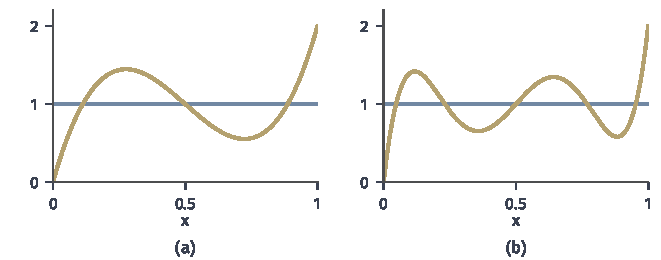
\includegraphics[width=112mm]{figures/07-probability/01-elementary-probability/matplotlib/rvm-same-moments/figure.pdf}
 \caption{前几个矩相同的不同密度。(a)常数密度$1$（蓝）与$1+q(x)$（黄），$q(x)=20x^{3}-30x^{2}+12x-1$，两者的前两阶矩相同；(b)常数密度与$1+252x^{5}-630x^{4}+560x^{3}-210x^{2}+30x-1$，前四阶矩相同。保持的矩越多，扰动振荡越快。}
 \label{fig:rvm-same-moments}
\end{BookInlineFigure}

那么全部矩能否确定分布？结论取决于尾部的轻重。取值有界时，全部矩确实决定分布，证明要用多项式在有界区间上一致逼近连续函数。尾部较重时则不然：存在各阶矩都有限且全部相同的两个不同分布，构造它们要用到第~\ref{chap:random-variable-transformations}章的密度换元，相关讨论可查阅~\scite{math-kallenberg2021probability}。用变换判断两个分布是否相同的系统工具在第~\ref{chap:weak-convergence-of-distributions}章介绍。在那之前，矩应当被看作分布的数值概括：它们回答特定的问题，例如平均、波动、偏斜，但不能代替概率表、分布函数或密度。
